\documentclass{article} 

\usepackage{graphicx}

\usepackage{subcaption} % for including subfigures

\begin{document}

Alan Mathison Turing was an English mathematician, computer scientist, logician, cryptanalyst, philosopher, and theoretical biologist. Turing was highly influential in the development of theoretical computer science, providing a formalisation of the concepts of algorithm and computation with the Turing machine, which can be considered a model of a general-purpose computer. He is widely considered to be the father of theoretical computer science and artificial intelligence. (from Wikipedia)

\begin{figure}[!htbp]
	\centering
    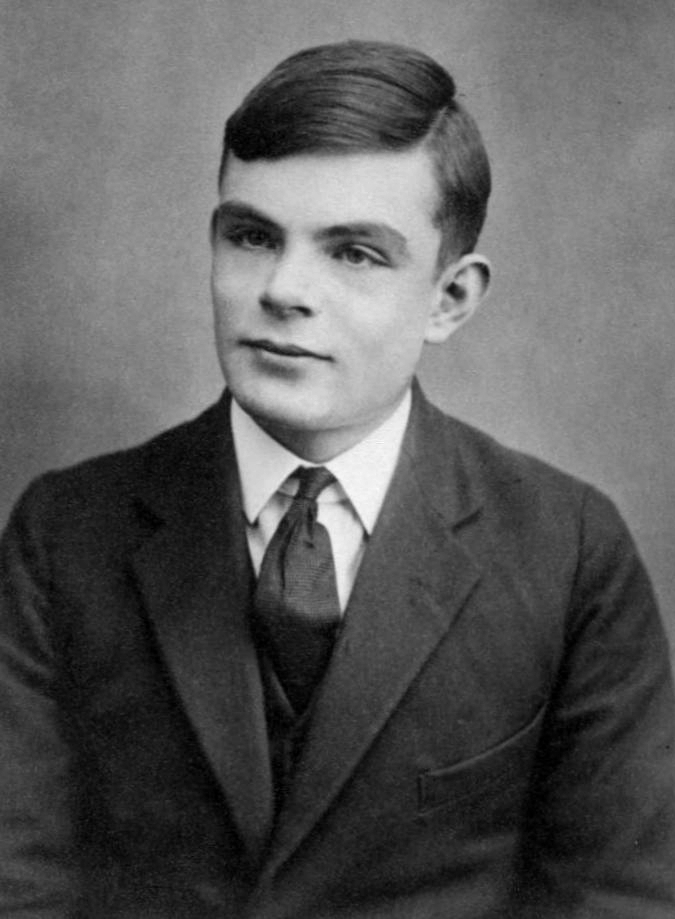
\includegraphics[width=0.5\linewidth]{Turing.jpeg}
    \caption{Alan Turing}
\end{figure}

\clearpage

Existentialism is a form of philosophical inquiry that explores the problem of human existence and centers on the subjective experience of thinking, feeling, and acting. For example, in the view of an existentialist, the individual's starting point has been called "the existential angst", a sense of dread, disorientation, confusion, or anxiety in the face of an apparently meaningless or absurd world. Existentialist thinkers frequently explore issues related to the meaning, purpose, and value of human existence. (from Wikipedia)

\begin{figure}[!t]
			\centering
			\begin{subfigure}[b]{0.4\textwidth}
				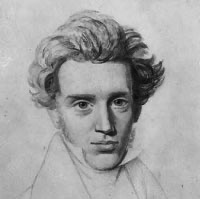
\includegraphics[width=\textwidth]{Kierkegaard}
				\caption{Kierkegaard}
			\end{subfigure}
			\begin{subfigure}[b]{0.4\textwidth}
				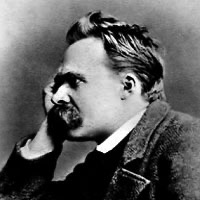
\includegraphics[width=\textwidth]{Nietzsche}
				\caption{Nietzsche}
			\end{subfigure}
			\\
			\begin{subfigure}[b]{0.4\textwidth}
				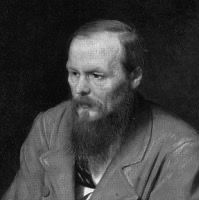
\includegraphics[width=\textwidth]{Dostoyevsky}
				\caption{Dostoyevsky}
			\end{subfigure}
			\begin{subfigure}[b]{0.4\textwidth}
				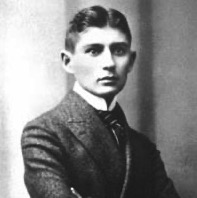
\includegraphics[width=\textwidth]{Kafka}
				\caption{Kafka}
			\end{subfigure}
			\caption{Existentialist philosophers}
		\end{figure}

\end{document}